\chapter{训练数据的生成与预处理}
\label{cha:usage-example}

\section{数据集的介绍}
本次项目采用的数据集为Skin Cancer MNIST: HAM10000。该数据集由10000张来自不同人群的皮肤镜图像组成。

数据集中的几张皮肤癌图片举例如图\ref{img401}。

\begin{figure}[h]
	\centering
	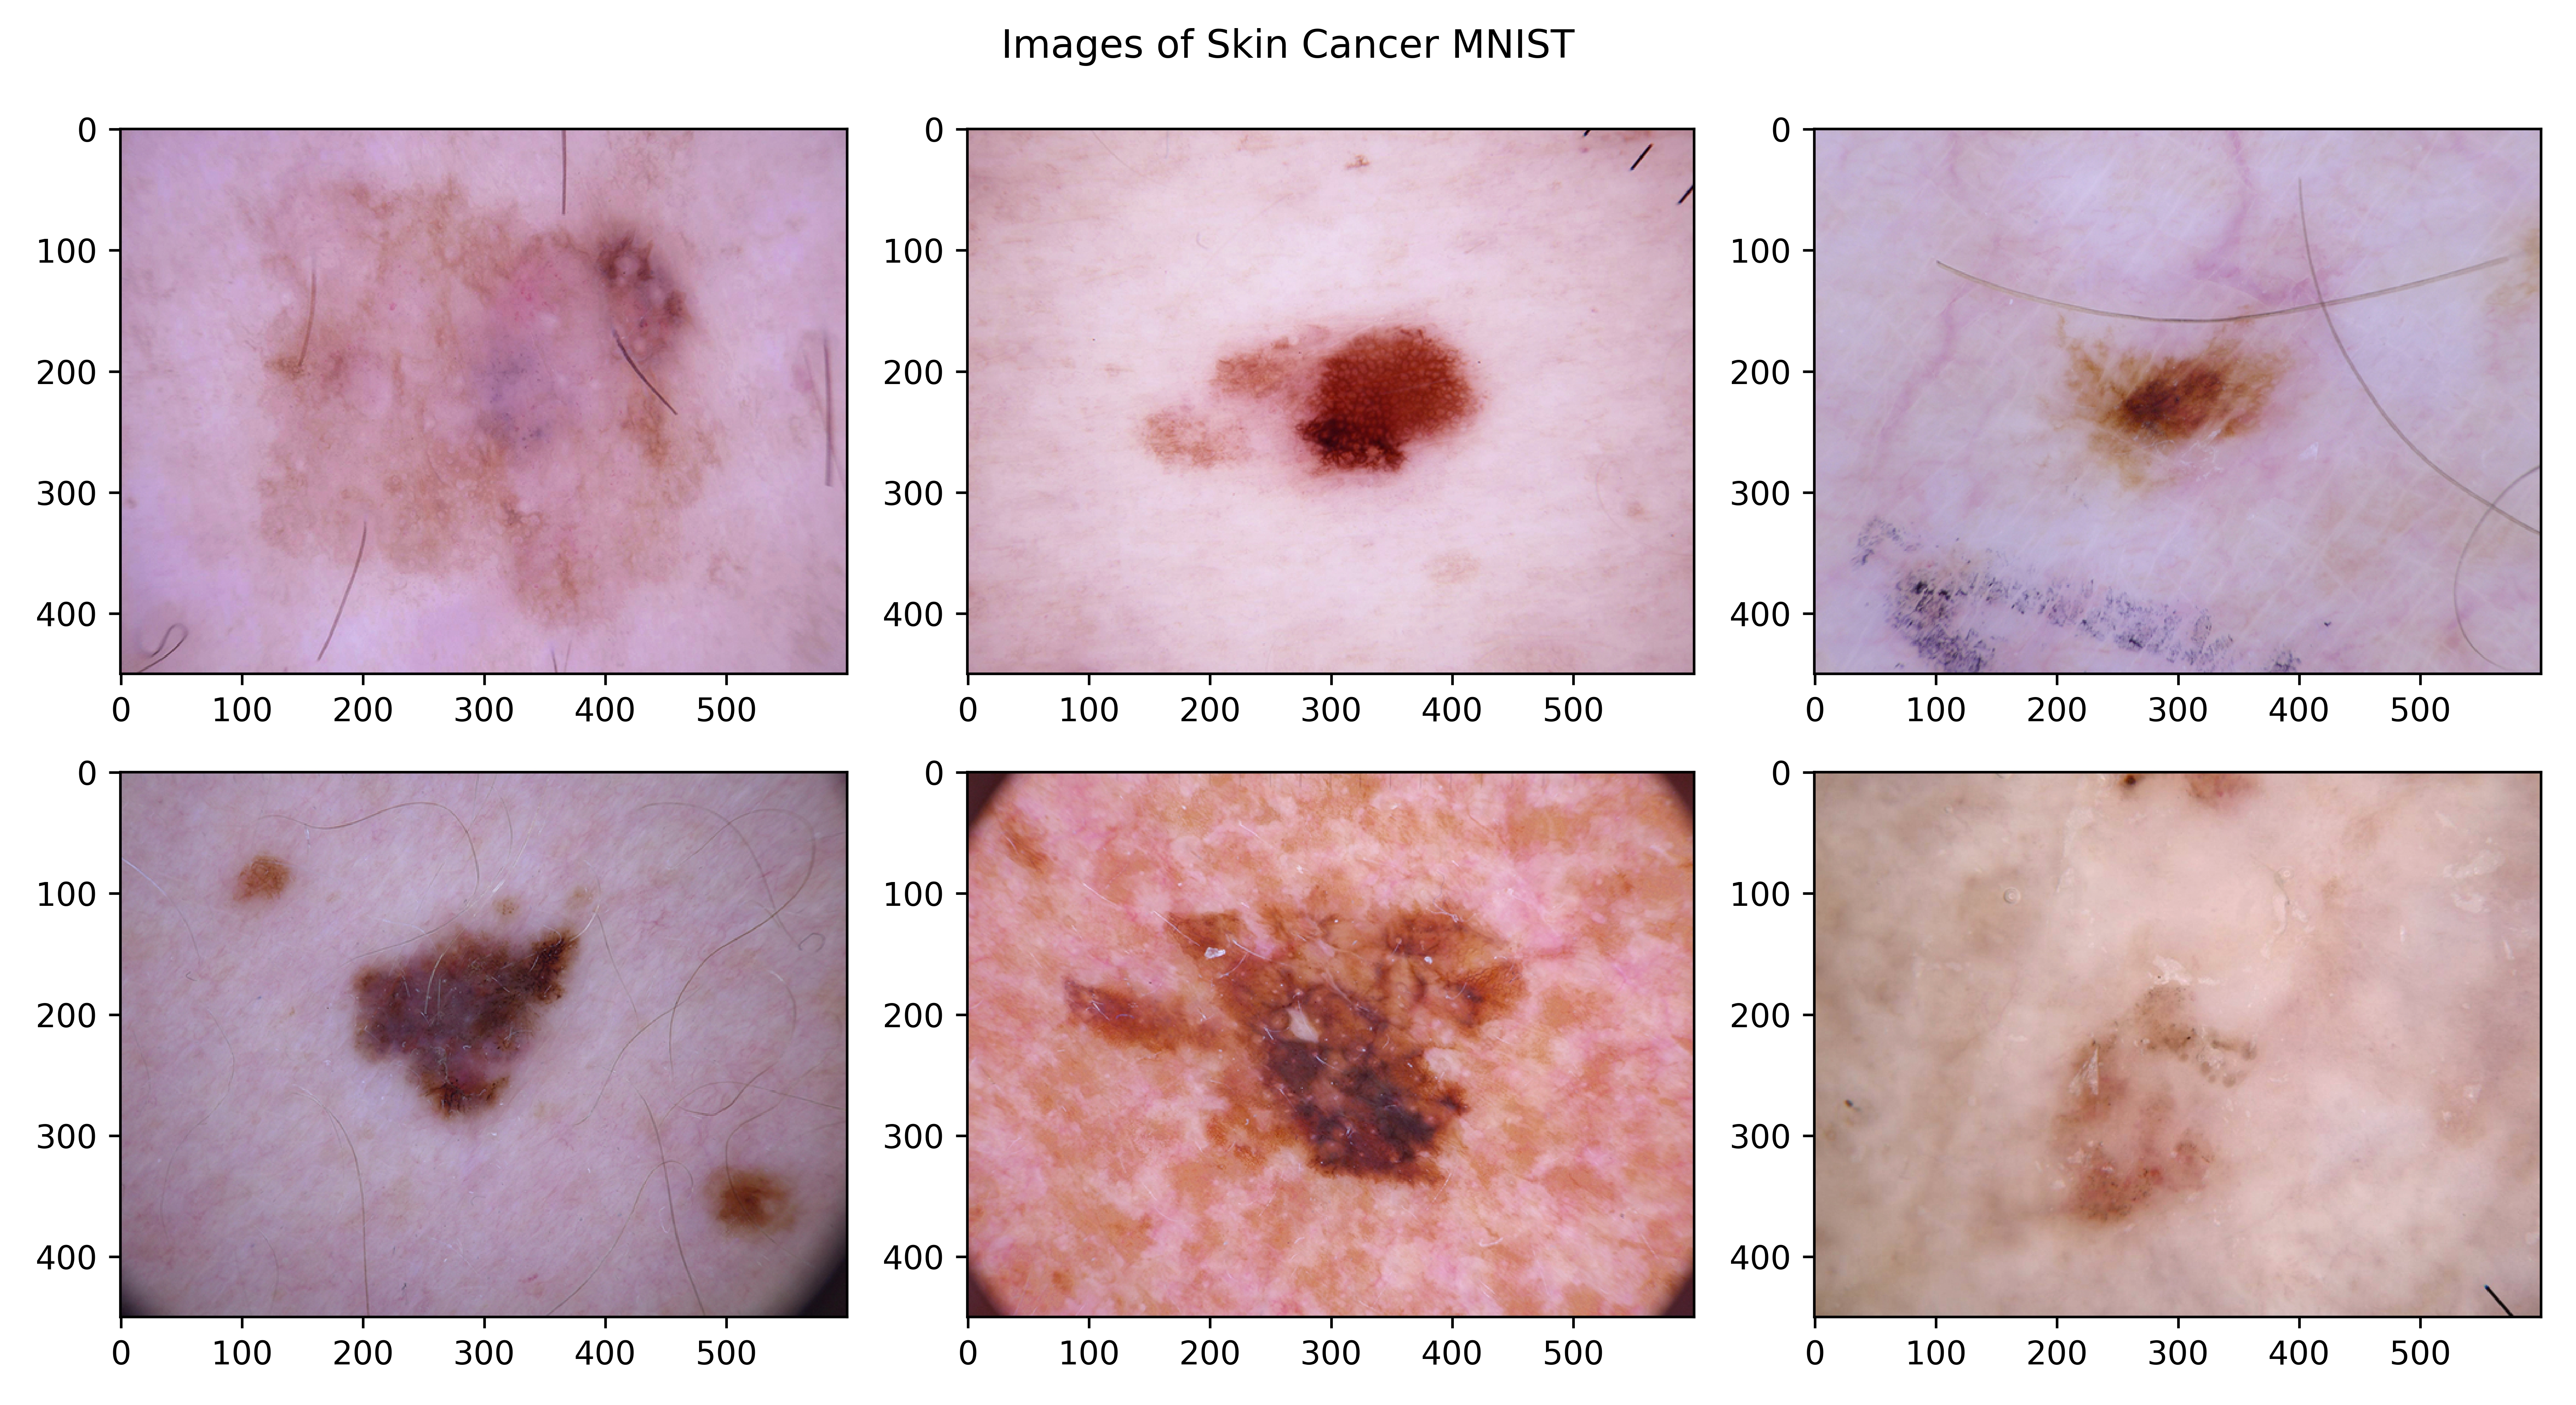
\includegraphics[width=0.9\columnwidth]{image/chap04/img401.png}
	\caption{Skin Cancer MNIST数据集示例}
	\label{img401}
\end{figure}

\section{k-wave的介绍与k空间伪谱法}
k-Wave是MATLAB的开源声学工具箱。该软件基于k空间伪谱法能实现复杂组织在真实介质中的声学仿真,并且还实现了多种对光声成像的重建方法。本项目采用该库实现对皮肤癌图像的光声成像仿真与重建。

\section{训练数据的生成与预处理}
下面介绍使用Skin Cancer MNIST数据集与k-Wave中的光声成像仿真与重建算法生成训练集与测试集的具体操作流程。

\subsection{在仿真前对Skin Cancer MNIST中的皮肤癌图像进行预处理}

\begin{enumerate}
	\item 读取图片并转为灰度图。
	\item 将图像归一化。由于用k-Wave进行模拟时外围填充的像素一定得是0,所以要在数据归一化的时候把原图里正常皮肤的部分对应到0。因此,取原图边界上的一些像素的平均值作为正常皮肤对应的像素值大小。然后在图像上将这个平均值映射到0;再在图像外围补上0像素点。
	\item 将图像降低分辨率(分辨率降低为原来的二分之一)。降采样的目的是使图像的分辨率变低,有效控制仿真的时间。
	\item 将图像的外围填充一圈0,目的是确保在光声成像模拟时,皮肤病灶完全位于圆形传感器阵列之中,使得光声成像模拟结果更加精确。
\end{enumerate}

下面选取Skin Cancer MNIST数据集中的一副皮肤癌图像对上述过程进行演示,如图\ref{img402}所示。

\begin{figure}[h]
	\centering
	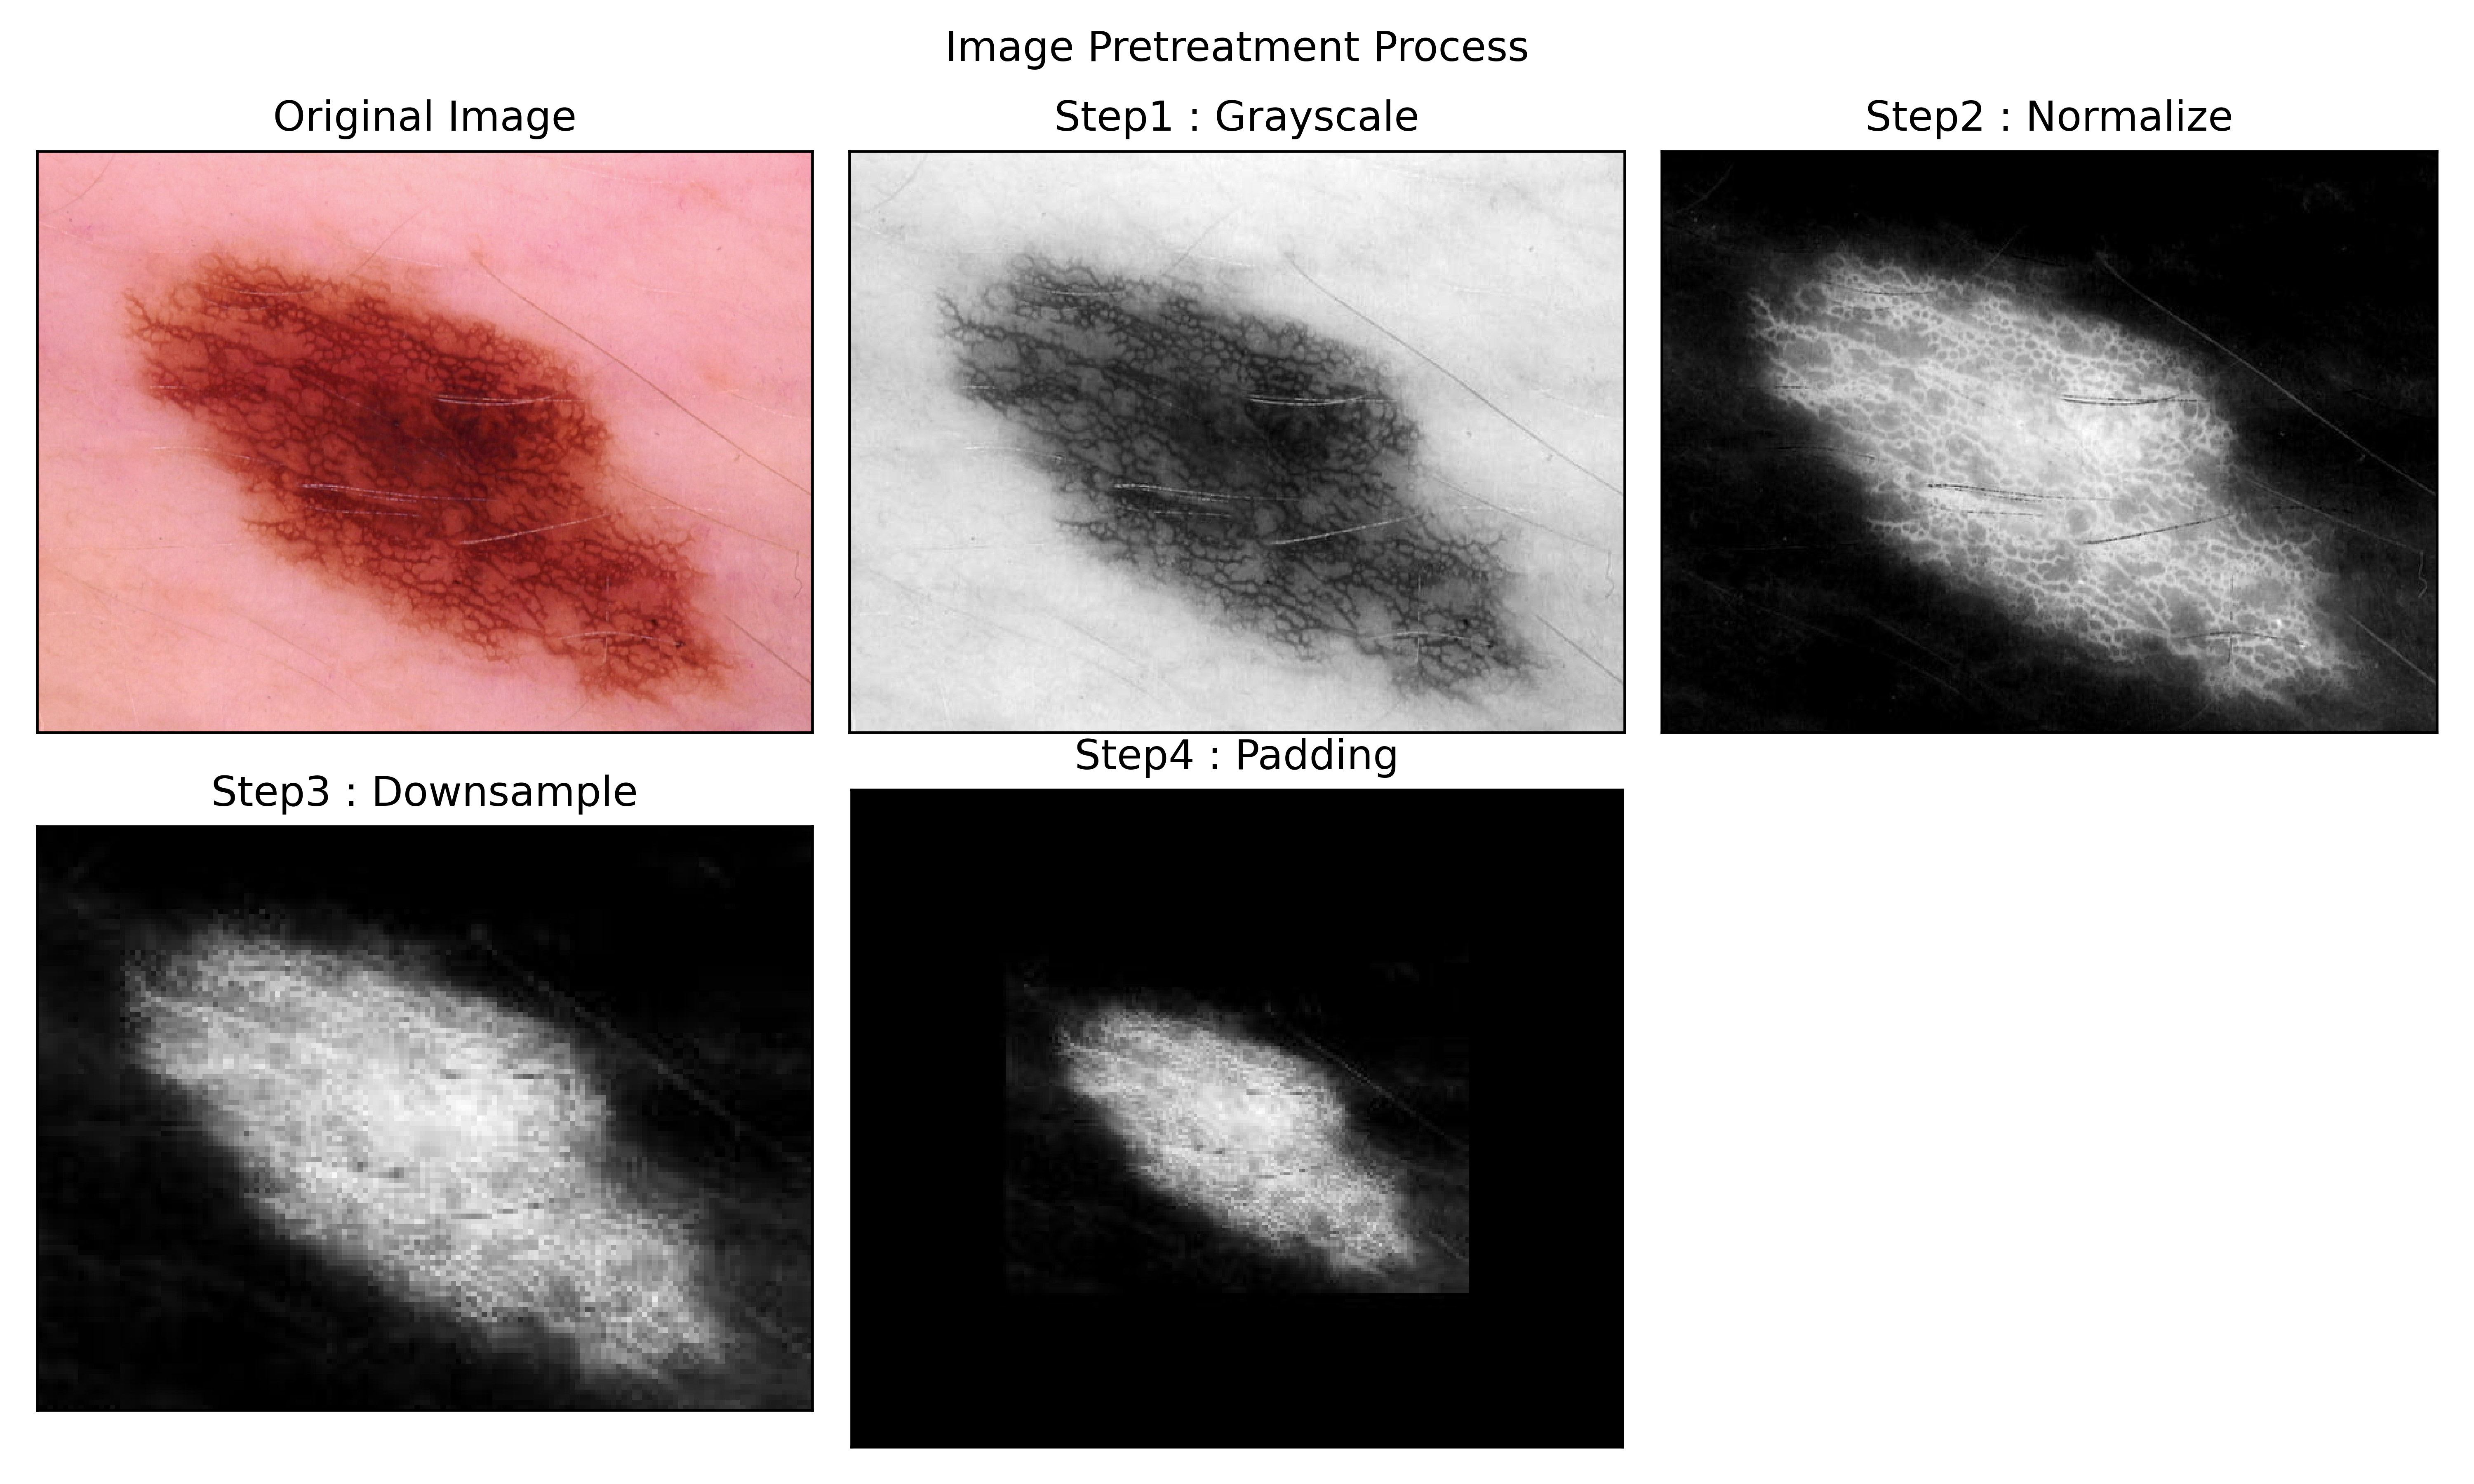
\includegraphics[width=0.9\columnwidth]{image/chap04/img402.png}
	\caption{预处理操作流程}
	\label{img402}
\end{figure}

\subsection{利用k-Wave对预处理后的图像进行光声成像仿真}
首先需要初始化k-Wave进行光声成像仿真各参数。在使用k-Wave进行光声成像模拟前,要设置的参数如图\ref{img403}所示。

\begin{figure}[h]
	\centering
	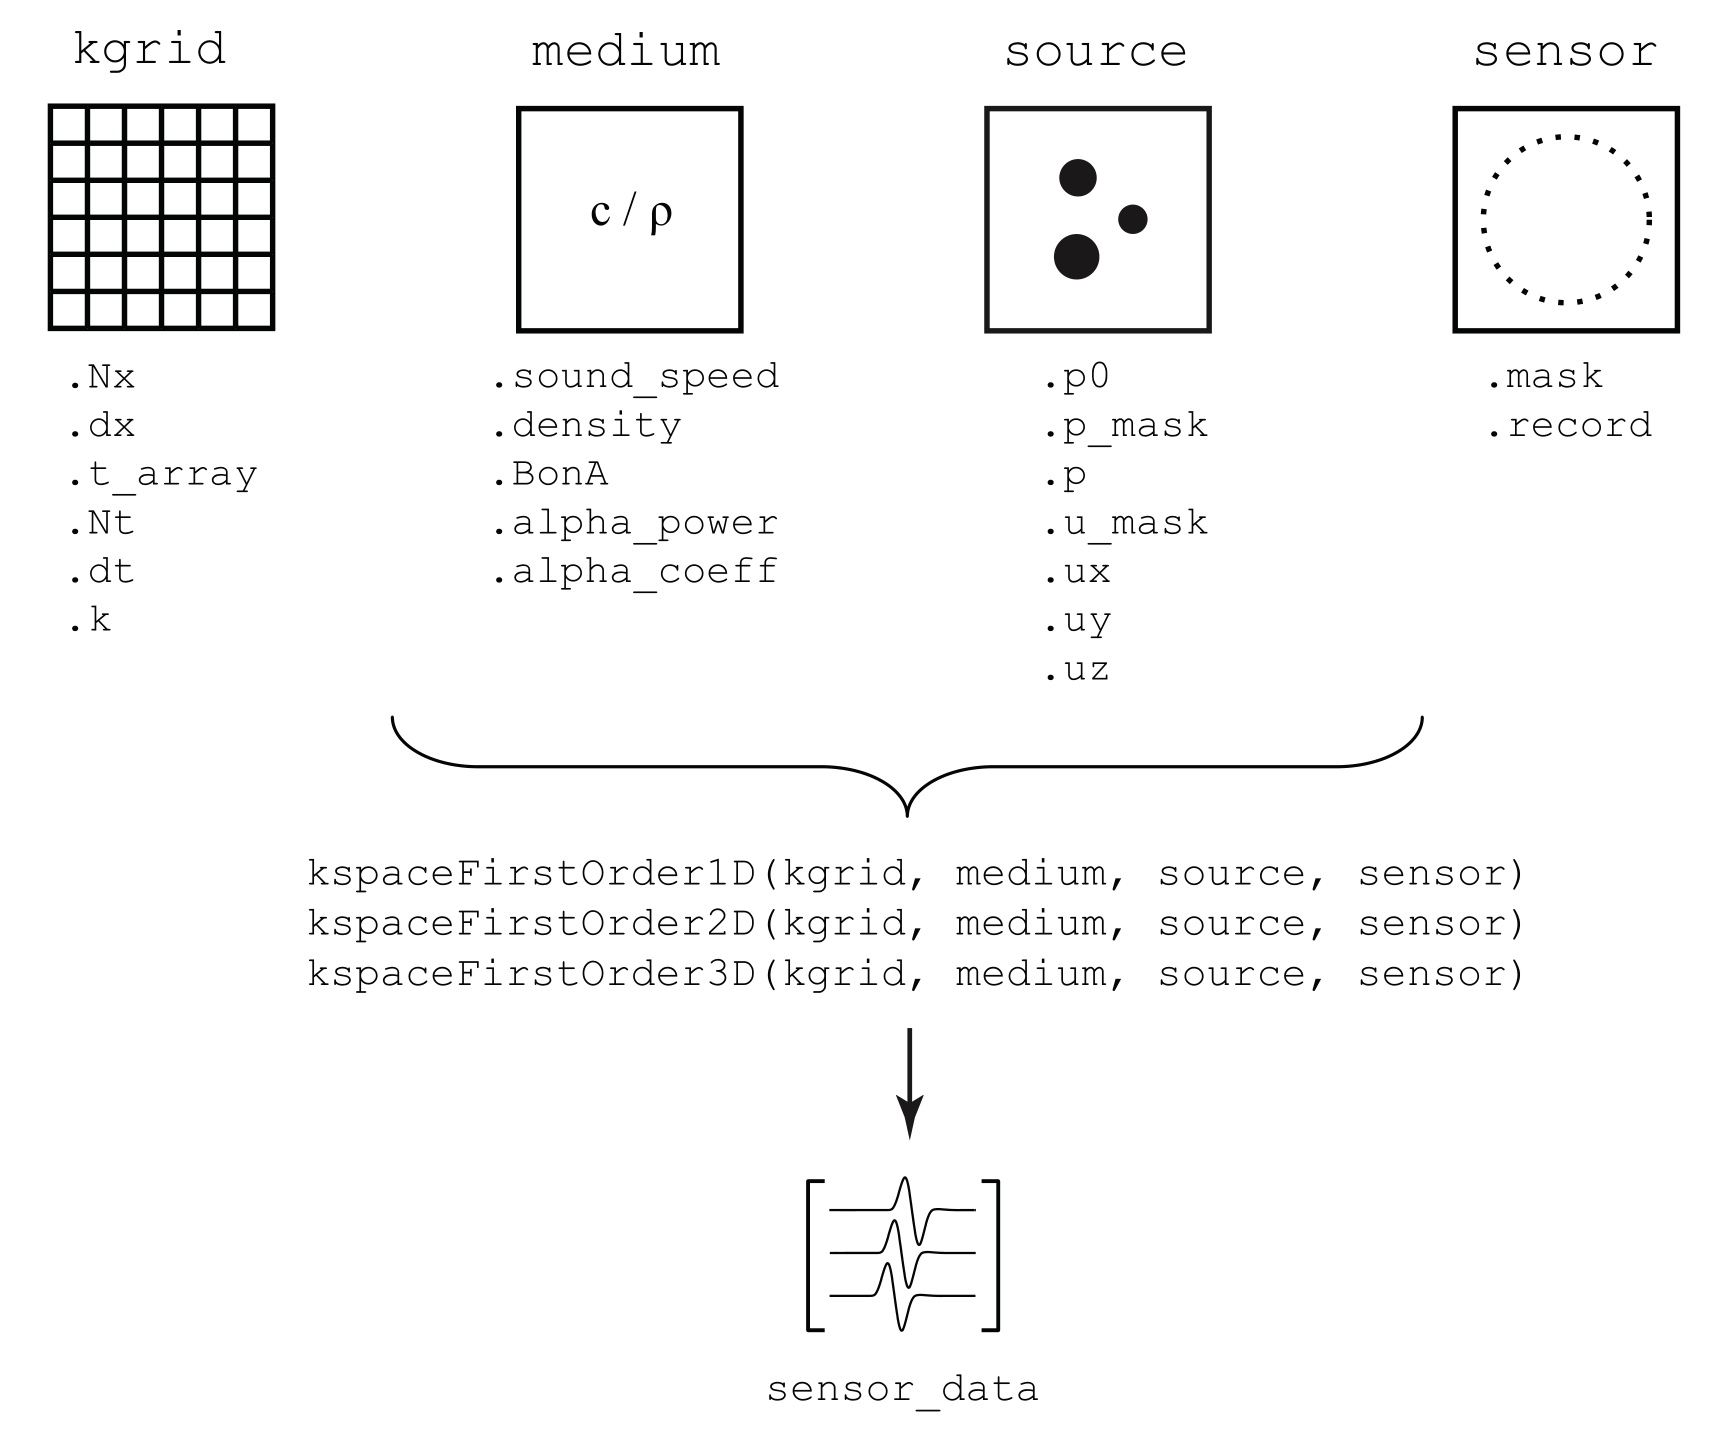
\includegraphics[width=0.6\columnwidth]{image/chap04/img403.png}
	\caption{k-Wave仿真的设置参数\cite{treeby2010k}}
	\label{img403}
\end{figure}
即创建计算网格、定义介质属性、定义初始压力、定义传感器掩模。

\begin{enumerate}
	\item 其中由于查资料得知:人体软组织声速接近1540m/s;2006年全国男人人体密度=$1.0913-0.0016\cdot (10.8+15.8)=1.0487\cdot 10^3kg/(m^3)$、女人人体密度=$1.0897-0.00133\cdot (17.5+17.5)=1.0431\cdot 10^3kg/(m^3)$。于是我设置介质声速为人体软组织声速,将男人人体密度与女人人体密度的平均值设置为介质密度。
	\item 将预处理好的图片导入模型中作为初始压力分布。
	\item 定义具有50个传感器元件的中心圆的笛卡尔传感器掩模
\end{enumerate}
在设置完如上参数后,利用MatLab运行kwave仿真。得出的输出数据senser data是形状为$[num\ sensor,time\ step]$的矩阵,记录了各传感器在各时间步长所接收到的压力数据。将其运用Matlab中的images函数做出图\ref{img404}。图片每一行代表着一个传感器在仿真过程中所接收到的压力的大小变化。

\begin{figure}[h]
	\centering
	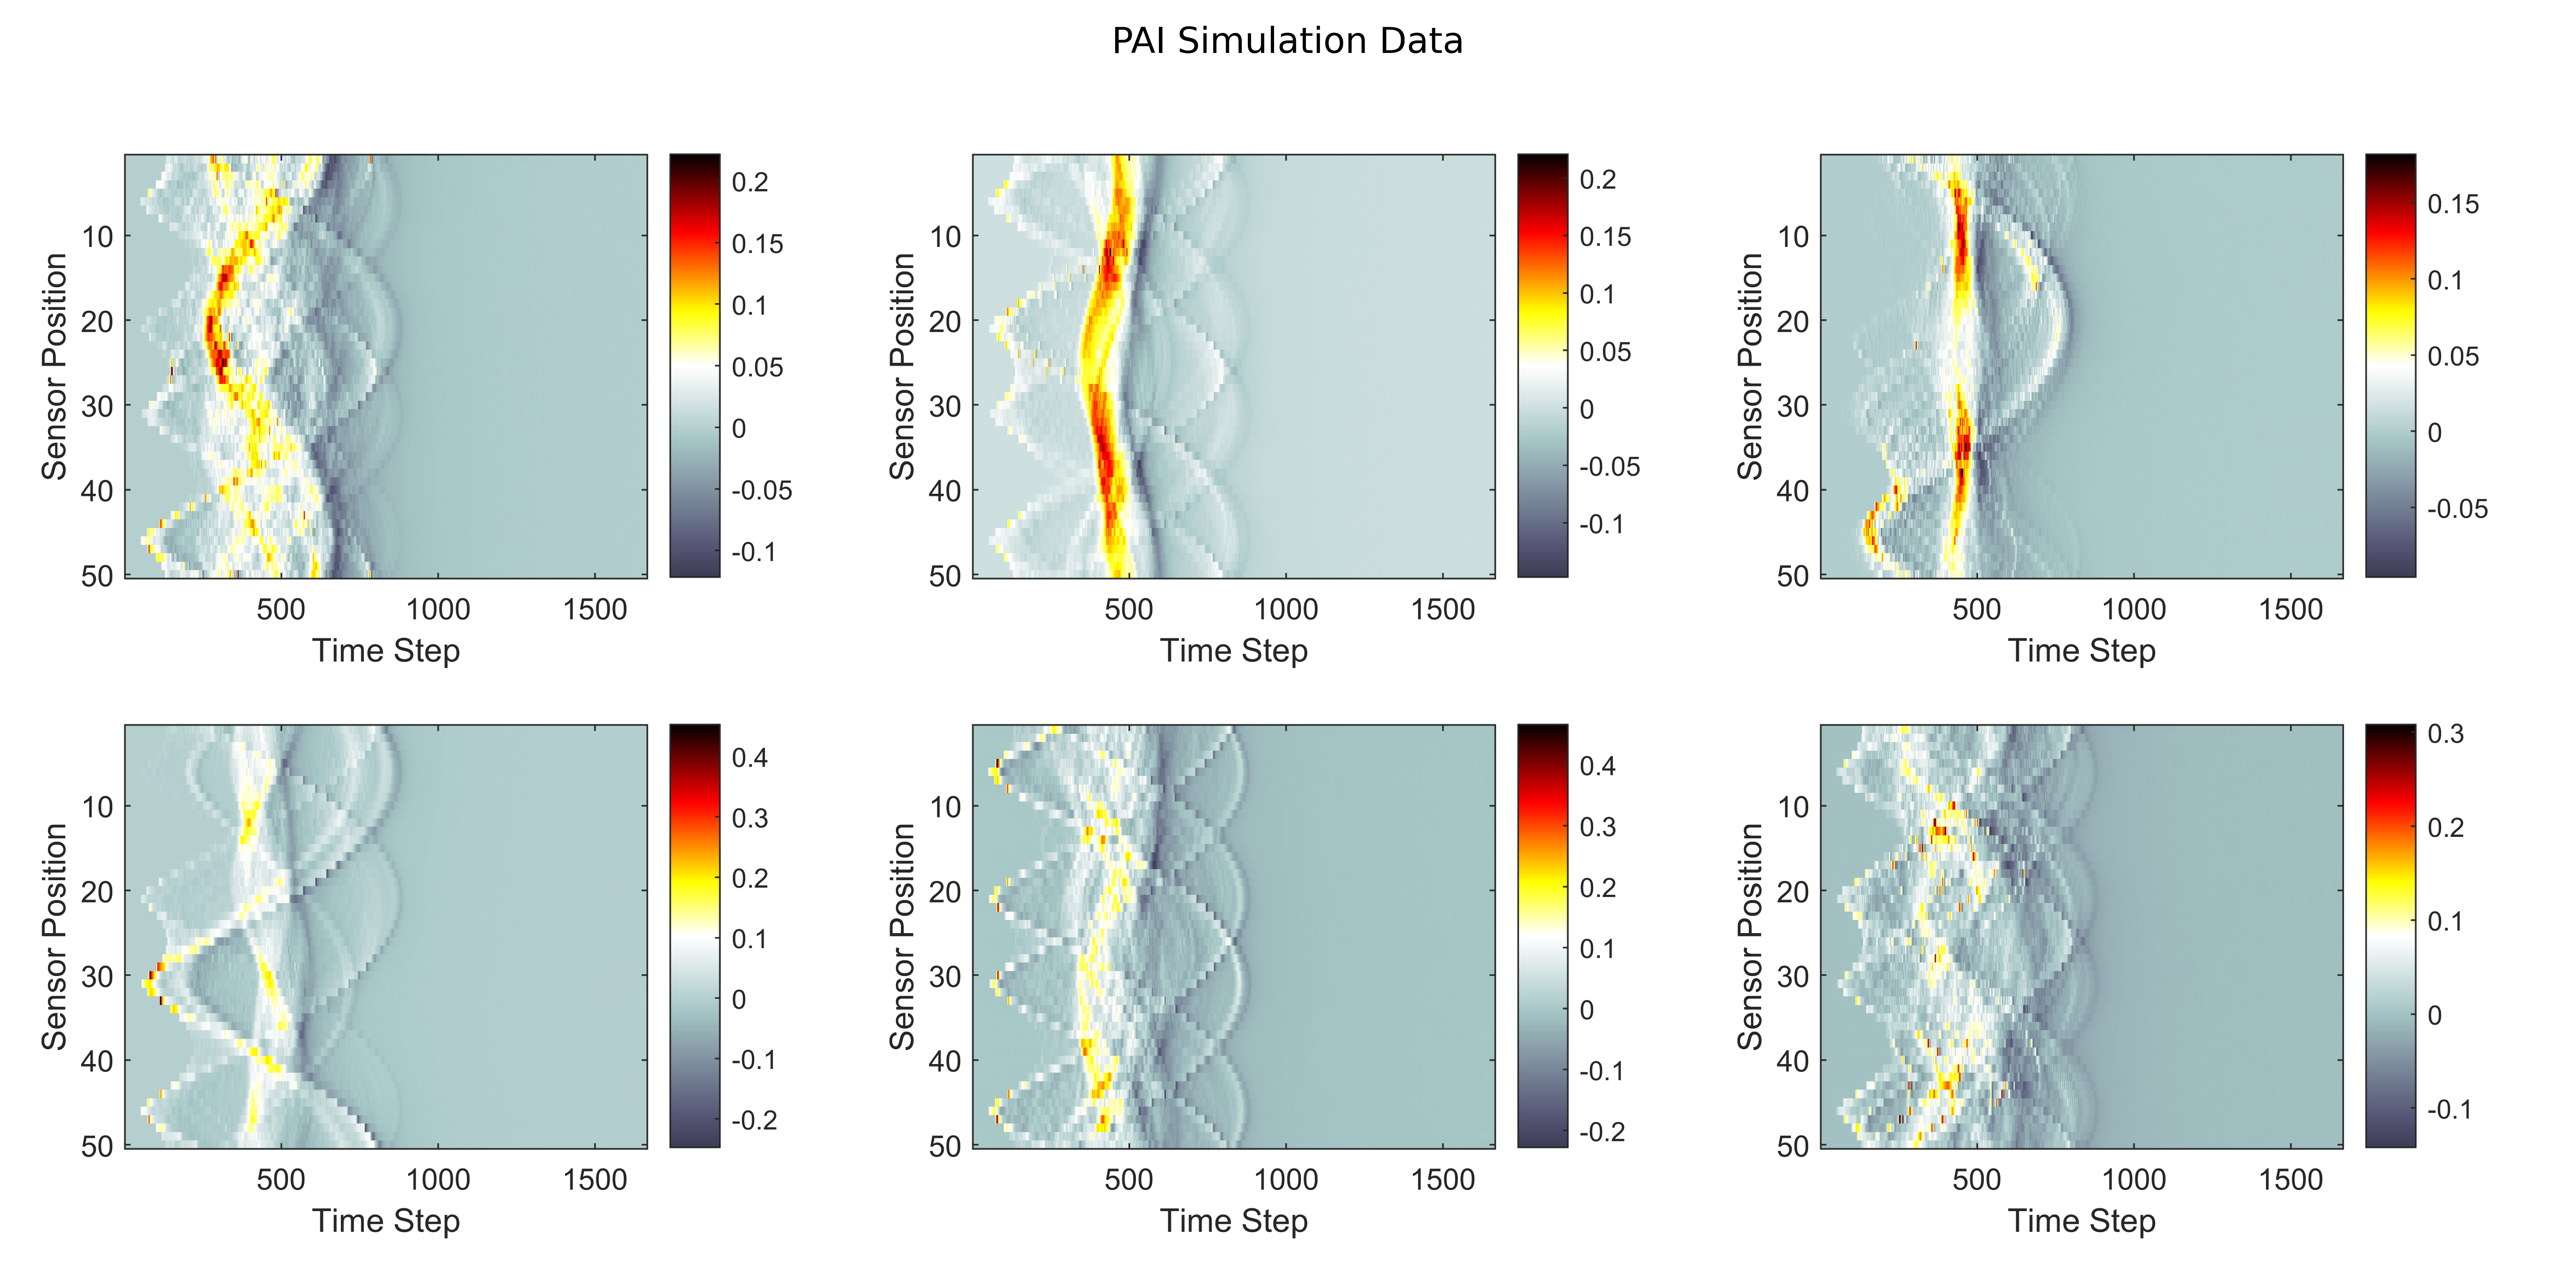
\includegraphics[width=0.9\columnwidth]{image/chap04/img404.png}
	\caption{光声传感器接收到的压力数据示例}
	\label{img404}
\end{figure}

\subsection{进行光声成像的重建得到训练数据}
在进行光声成像重建前,同样需要初始化k-Wave的各项参数,并且确保其与仿真时保持一致;然后才能使用k-Wave中的相关函数进行光声成像的重建。重建图像如图所示\ref{img405}。其中左侧为原图像,右侧为相应的重建图像。

\begin{figure}[h]
	\centering
	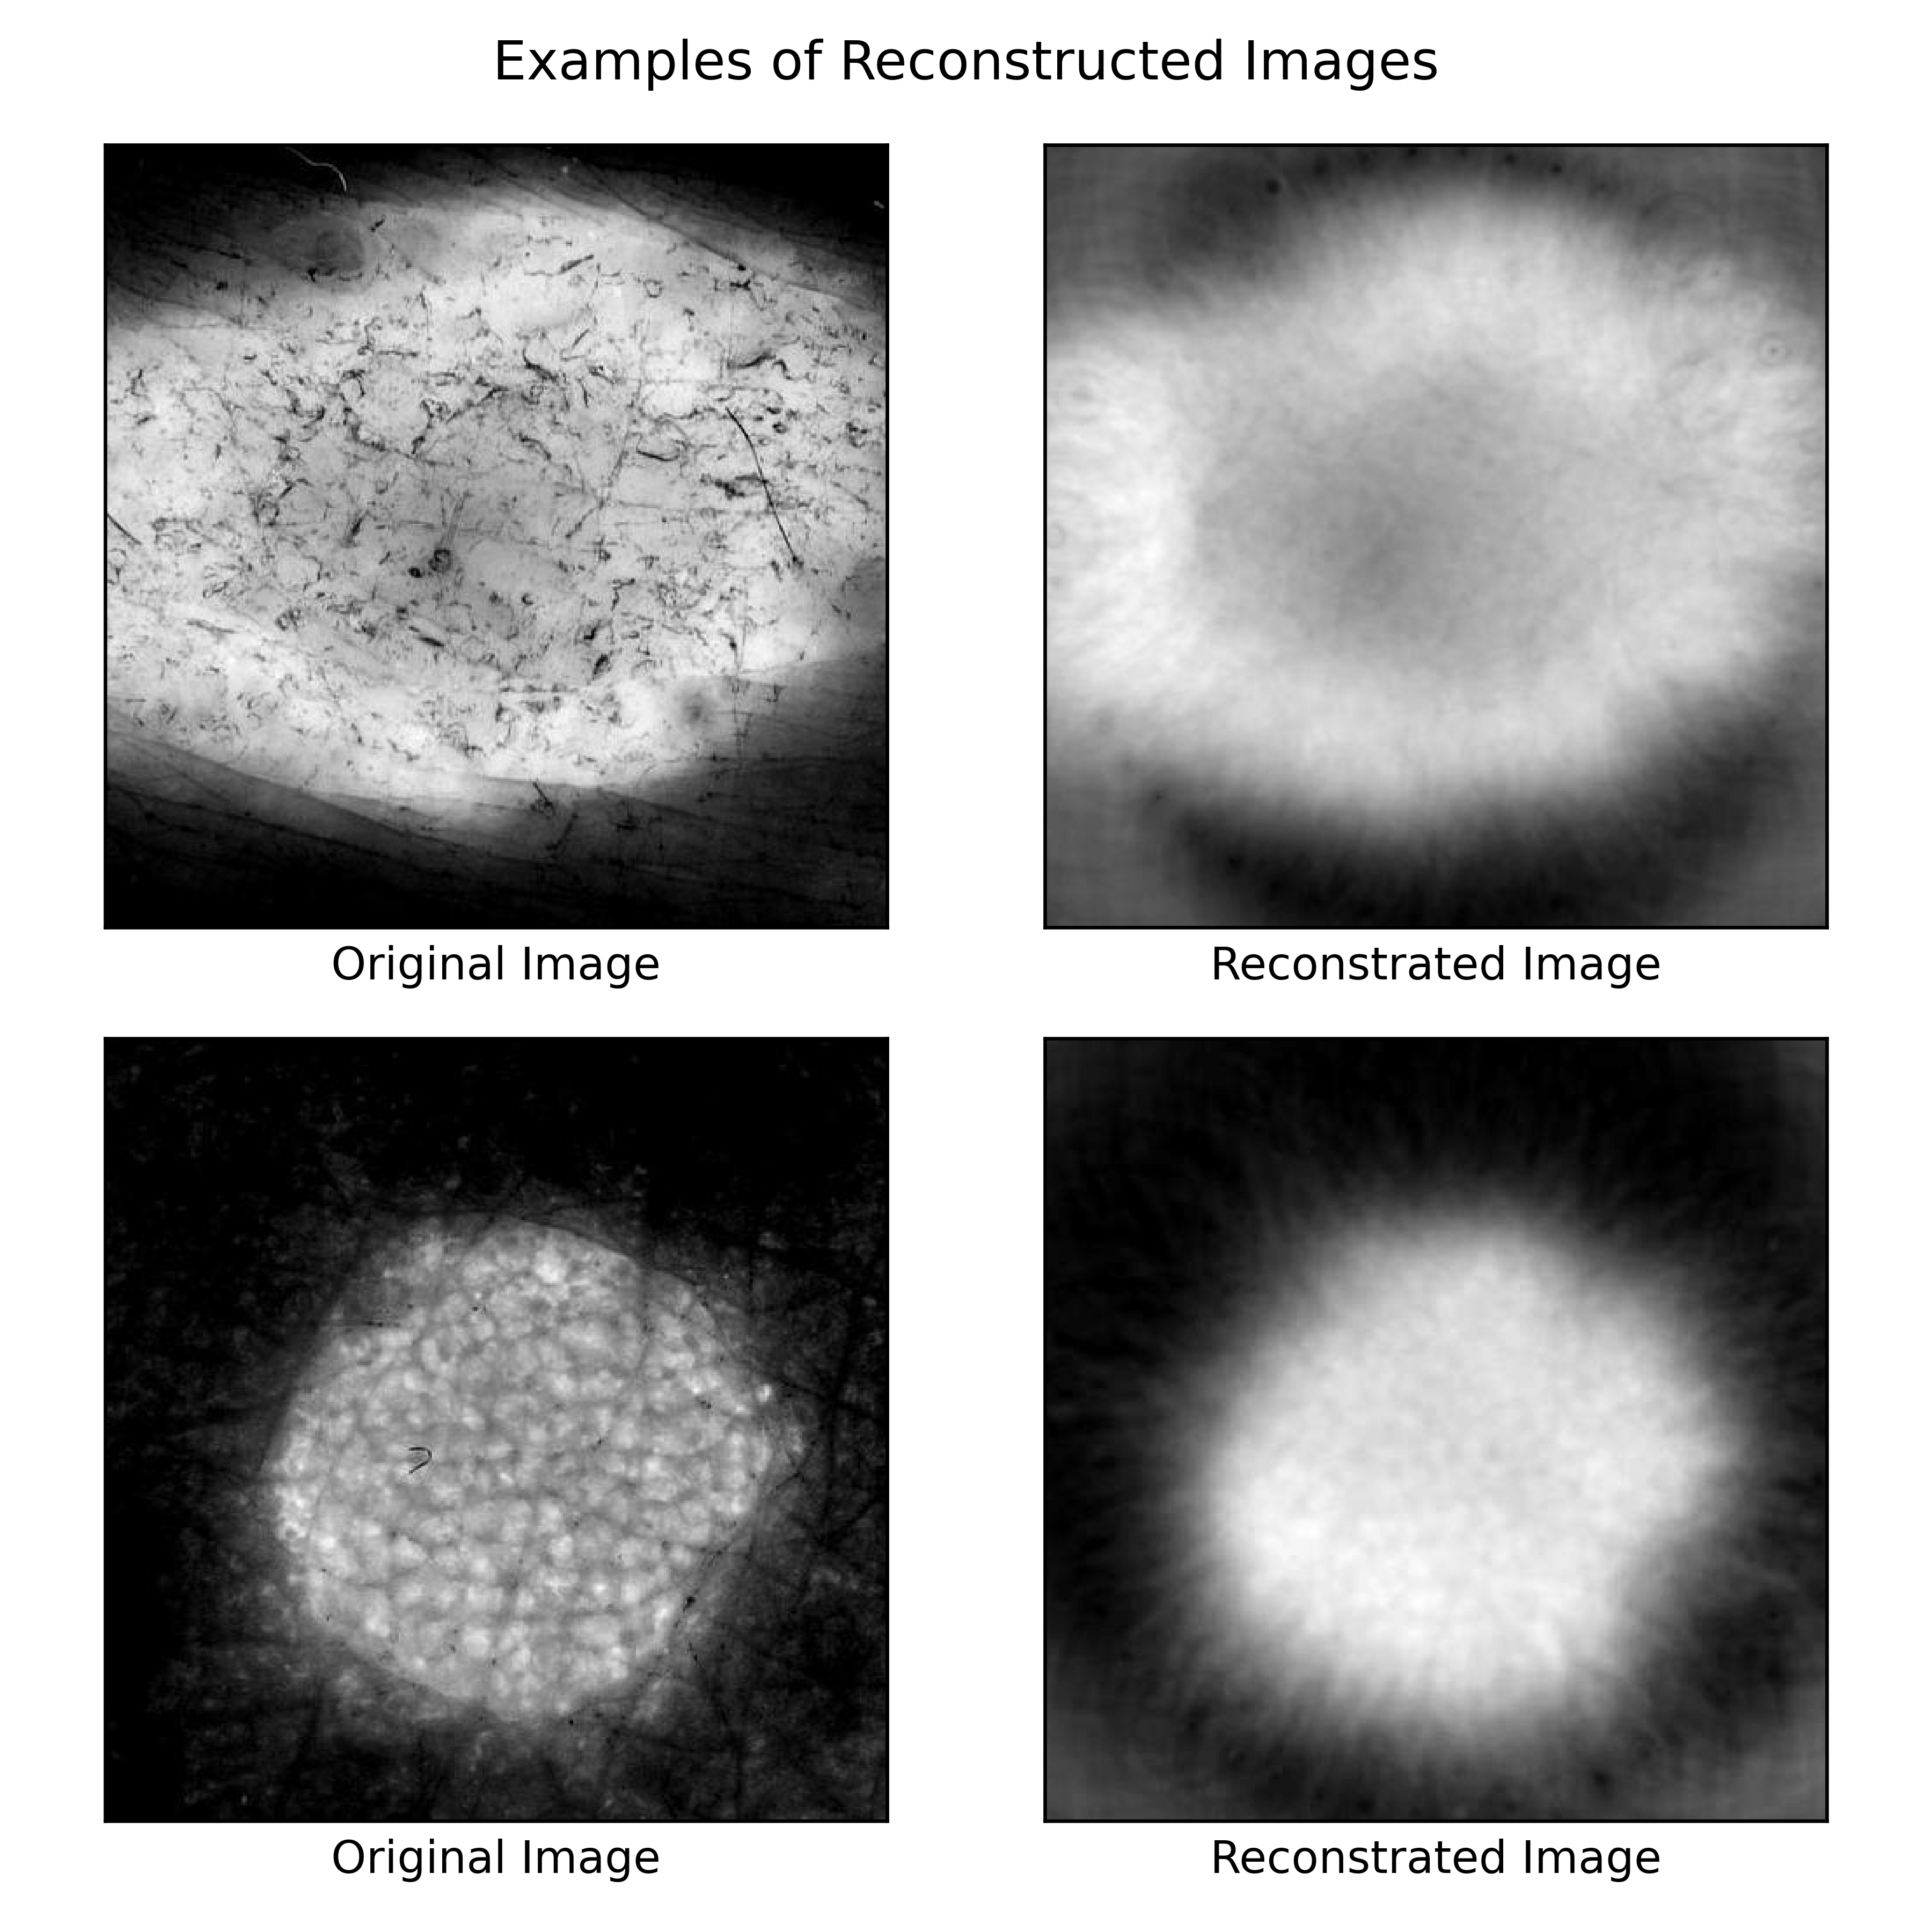
\includegraphics[width=0.75\columnwidth]{image/chap04/img405.png}
	\caption{重建图像示例}
	\label{img405}
\end{figure}

\subsection{将得到的数据集划分成训练集及测试集}
经过上述光声成像仿真与重建,最终共得到6000张重建图像。将其中的5000张重建图像及其原图像划分为训练集,将其余的1000张重建图像及其原图像划分为测试集。